\documentclass[main.tex]{subfiles}
\begin{document}
\begin{enumerate}
% -----------------------------------------------------
% Ex 1 
% -----------------------------------------------------
\item{A spherical wave and a plane wave (same wavelength) are co-propagating on axis in air as shown in Figure \ref{fig:51}.}

\begin{figure}
\centering\fbox{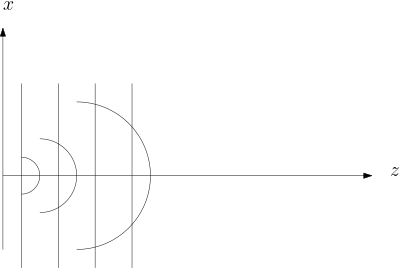
\includegraphics[height=2.0in]{figures/hw5/hw5_1.png}}
\caption{Propagating Spherical Wave and Planar Wave}
\label{fig:51}
\end{figure}

The energy of a plane wave wave $E_{\mathrm{pl}}$ and the energy of a spherical wave $E_{\mathrm{sp}}$ are defined in Equation \ref{eq:51} where $\alpha = $.

\begin{equation}\label{eq:51}
\begin{array}{l}
{E_{\mathrm{pl}}=\left|E_{\mathrm{pl}}\right| e^{i \frac{2 \pi}{\lambda} z}} \\
{E_{\mathrm{sp}}=\frac{\left|E_{\mathrm{sp}}\right|}{\alpha z} e^{i \frac{2 \pi}{\lambda} z} e^{i \pi \frac{\left(x^{2}+y^{2}\right)}{\lambda z}}}
\end{array}
\end{equation}

\begin{enumerate}
\item Describe the interference pattern observed at $z=100\lambda$ from the origin of spherical wave.

At $z=100\lambda$, assuming the amplitudes $A$ of the two waves are equal we can define the phase difference between the waves in Equation \ref{eq:52}. 

\begin{equation}\label{eq:52}
\begin{array}{l}
{E_{\mathrm{pl}}=e^{i \phi_{\mathrm{pl}}} \text { where } \phi_{\mathrm{pl}}=\frac{2 \pi}{\lambda} z} \\ 
{E_{\mathrm{sp}}=e^{i \phi_{\mathrm{sp}}} \text { where } \phi_{\mathrm{sp}}=\frac{2 \pi}{\lambda} z+\frac{\pi}{\lambda z}\left(x^{2}+y^{2}\right)} \\ 
{\Delta \phi=\phi_{\mathrm{sp}}-\phi_{\mathrm{pl}}=\frac{\pi}{\lambda z}\left(x^{2}+y^{2}\right)}\end{array}
\end{equation}

The bright interference fringes occur where $\Delta \phi=2 \pi m, m=0,1,2 \ldots$ when the two waves are in phase and $\therefore  \frac{x^{2}+y^{2}}{2 z}=m \lambda$  At $z=100 \lambda \rightarrow x^{2}+y^{2}=200 \lambda^{2} m, m=0,1,2,3 \ldots $, using the circle equation $(x-x_{O})^{2}+(y-y_{O})^{2}=r^2$ from the origin we can solve for the interference pattern which is a set of concentric rings of radii $R=\lambda \sqrt{200 m}, m=0,1,2,3 \ldots$

\begin{figure}
\centering\fbox{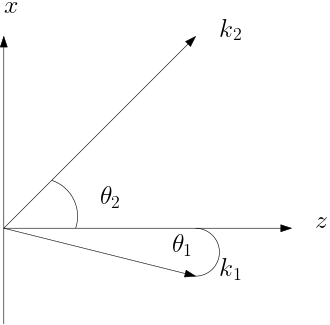
\includegraphics[height=2.0in]{figures/hw5/hw5_1b.png}}
\caption{Off-axis co-propagating plan waves}
\label{fig:52}
\end{figure}

\item Describe the interference pattern for an off-axis co-propagating plane wave ($\theta_1 = -30$ degrees and $\theta_2 = +45$ degrees in the xz plane with respect to z) as shown in Figure \ref{fig:52}.

The energy of a plane waves $E_{\mathrm{pl1}}$ and $E_{\mathrm{pl1}}$ are defined in Equation \ref{eq:53}.

\begin{equation}\label{eq:53}
\begin{array}{l}
{E_{\mathrm{pl1}}=\left|E_{\mathrm{pl1}}\right| e^{i \frac{2 \pi}{\lambda}(x \sin \theta_1+z \cos \theta_1)}}\\
{E_{\mathrm{pl2}}=\left|E_{\mathrm{pl2}}\right| e^{i \frac{2 \pi}{\lambda}(x \sin \theta_2+z \cos \theta_2)}}
\end{array}
\end{equation}

Assuming the amplitudes $A$ are equal at $z=100\lambda$, and intensity $I=2\left|E_{\mathrm{pl}}\right|^{2}(1+\cos \Delta \phi)$, we calculate phase delta $\Delta \phi=\phi_{\mathrm{pl2}}-\phi_{\mathrm{pl1}}$ in Equation \ref{eq:54}.

\begin{equation}\label{eq:54}
\Delta \phi= \frac{2 \pi}{\lambda} \left((x \sin \theta_2+z \cos \theta_2) - (x \sin \theta_1+z \cos \theta_1) \right)
\end{equation}

Bright fringes occur when $\Delta \phi = 2\pi m$, $m=1,2,3,\cdot$ which allows us to calculate the interference pattern in Equation \ref{eq:55}.

\begin{equation}\label{eq:55}
\lambda m =  x(\sin(45)-\sin(-30)) + z(\cos(45)-\cos(-30))
\end{equation}

\item Is it possible to generate this kind of wave with a Michelson Interferometer? Please motivate and describe your answer extensively.
\end{enumerate}
% -----------------------------------------------------
% Ex 2 
% -----------------------------------------------------
\item{Consider a sinusoidal amplitude grating.}
$$g_t(x)=\frac{1}{2}\left[ 1+m\cos(\frac{2\pi x}{A}) + \phi) \right]$$
at $z=0$. Illuminated by an off-axis plane wave.
$$g(x,z=0)=\exp(\frac{2\pi}{\lambda}i \theta x)$$
\begin{enumerate}
\item{Derive the expression of $g_{\text{+}}(x,z=0)$}
\item{What would be the interference pattern at infinity (Today's lecture)}
\end{enumerate}
% -----------------------------------------------------
% Ex 3 
% -----------------------------------------------------
\item{Derive the interference pattern of a plane wave passing through a double split for $D=10\lambda$. Use Huygens' principle and derive the superposition of the waves at a distance $z=L$.}
\end{enumerate}
\end{document}